\documentclass[a4paper,12pt]{book}
\usepackage[utf8]{inputenc}
\title{}
\author{Rachel Morris}
\date{\today}

\usepackage{rachwidgets}
\usepackage{fancyhdr}
\usepackage{lastpage}
\usepackage{dirtree}
\usepackage{boxedminipage}
\usepackage{colortbl} % cell bg colors

\setcounter{chapter}{4}
\setcounter{section}{2}
\newcommand{\laChapter}{4.3 Properties of Functions and Set Cardinality\ }
\newcounter{question}

\newcommand{\laClass}{CS 210\ }
\newcommand{\laSemester}{Fall 2017\ }

\pagestyle{fancy}
\fancyhf{}
\lhead{\laClass \laSemester}
\chead{}
\rhead{Ch \laChapter}
\rfoot{\thepage\ of \pageref{LastPage}}
\lfoot{\scriptsize Compiled by Rachel Morris, last updated \today}

\renewcommand{\headrulewidth}{2pt}
\renewcommand{\footrulewidth}{1pt}

\begin{document}

    %\toggletrue{answerkey}
    \togglefalse{answerkey}

    %------------------------------------------------------------------%
    %- Exercise Begin -------------------------------------------------%
    %------------------------------------------------------------------%

    \section{Properties of Functions and Set Cardinality}

    \subsection{Review: Inverses of functions}

    \notonkey{
        \begin{introNOHEAD}{}
            Given a relation $R$ with domain $A$ and codomain $B$,
            the relation $R_{-1}$ (read ``$R$ inverse") with domain $B$
            and codomain $A$ is called the \textbf{inverse} of $R$,
            and is defined so that
            \begin{center}
                $(x,y) \in R$ \tab if and only if \tab $(y,x) \in R^{-1}$
            \end{center}

            Also note that the inverse of $R^{-1}$ is $R$.
            \footnote{Discrete Mathematics, Ensley and Crawley}
        \end{introNOHEAD}
    }{}

    
    
    % -------------------------------------------------------------%
    % - QUESTION --------------------------------------------------%
    % -------------------------------------------------------------%
    \stepcounter{question}
    \begin{questionNOGRADE}{\thequestion}

        Draw the inverse of each diagram. Identify whether the original
        diagram and/or the inverse of that diagram are functions. ~\\

        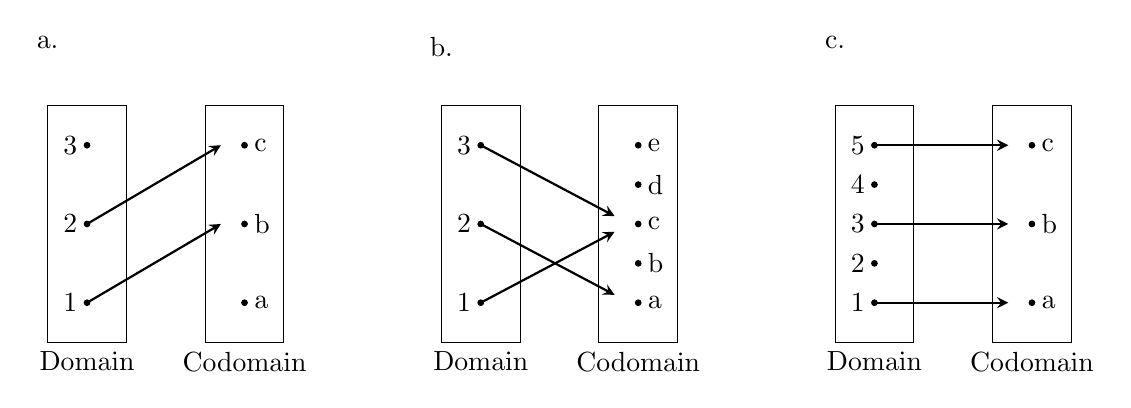
\begin{tikzpicture}[arrow/.style = {thick,-stealth}]
            % Graph 1
            \node [below] at (0,4) {a.};
            
            \draw (0,0) rectangle (1,3);
            \draw (2,0) rectangle (3,3);
            
            \node [below] at (0.5,0) {Domain};
            \node [below] at (2.5,0) {Codomain};

            \filldraw (0.5, 0.5) circle (1pt) node[left] {1};
            \filldraw (0.5, 1.5) circle (1pt) node[left] {2};
            \filldraw (0.5, 2.5) circle (1pt) node[left] {3};

            \filldraw (2.5, 0.5) circle (1pt) node[right] {a};
            \filldraw (2.5, 1.5) circle (1pt) node[right] {b};
            \filldraw (2.5, 2.5) circle (1pt) node[right] {c};
            
            \draw[arrow] (0.5, 0.5) -- (2.2, 1.5);
            \draw[arrow] (0.5, 1.5) -- (2.2, 2.5);

            % Graph 2
            \node [below] at (5,4) {b.};
            
            \draw (5,0) rectangle (6,3);
            \draw (7,0) rectangle (8,3);
            
            \node [below] at (5.5,0) {Domain};
            \node [below] at (7.5,0) {Codomain};

            \filldraw (5.5, 0.5) circle (1pt) node[left] {1};
            \filldraw (5.5, 1.5) circle (1pt) node[left] {2};
            \filldraw (5.5, 2.5) circle (1pt) node[left] {3};

            \filldraw (7.5, 0.5) circle (1pt) node[right]   {a};
            \filldraw (7.5, 1) circle (1pt) node[right]     {b};
            \filldraw (7.5, 1.5) circle (1pt) node[right]   {c};
            \filldraw (7.5, 2) circle (1pt) node[right]     {d};
            \filldraw (7.5, 2.5) circle (1pt) node[right]   {e};
            
            \draw[arrow] (5.5, 0.5) -- (7.2, 1.4);
            \draw[arrow] (5.5, 2.5) -- (7.2, 1.6);
            \draw[arrow] (5.5, 1.5) -- (7.2, 0.6);

            % Graph 3
            \node [below] at (10,4) {c.};
            
            \draw (10,0) rectangle (11,3);
            \draw (12,0) rectangle (13,3);
            
            \node [below] at (10.5,0) {Domain};
            \node [below] at (12.5,0) {Codomain};

            \filldraw (10.5, 0.5) circle (1pt) node[left]   {1};
            \filldraw (10.5, 1) circle (1pt) node[left]     {2};
            \filldraw (10.5, 1.5) circle (1pt) node[left]   {3};
            \filldraw (10.5, 2) circle (1pt) node[left]     {4};
            \filldraw (10.5, 2.5) circle (1pt) node[left]   {5};

            \filldraw (12.5, 0.5) circle (1pt) node[right] {a};
            \filldraw (12.5, 1.5) circle (1pt) node[right] {b};
            \filldraw (12.5, 2.5) circle (1pt) node[right] {c};

            \draw[arrow] (10.5,0.5) -- (12.2,0.5);
            \draw[arrow] (10.5,1.5) -- (12.2,1.5);
            \draw[arrow] (10.5,2.5) -- (12.2,2.5);
        \end{tikzpicture}

        \solution{
            ~\\ ~\\
            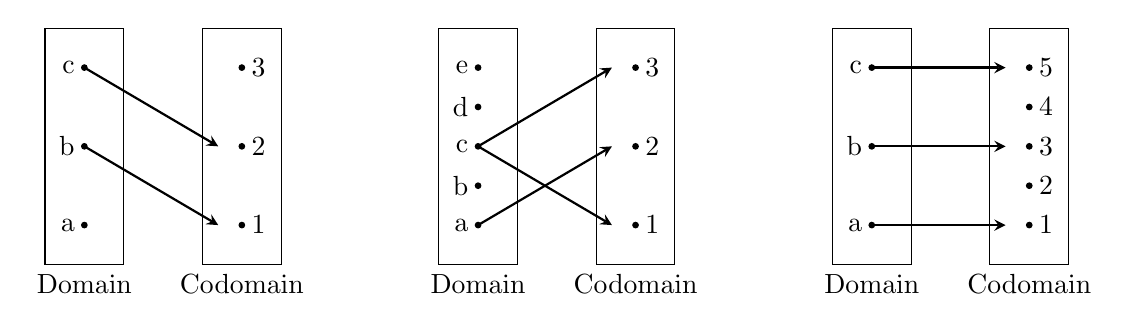
\begin{tikzpicture}[arrow/.style = {thick,-stealth}]
                % Graph 1
                
                \draw (0,0) rectangle (1,3);
                \draw (2,0) rectangle (3,3);
                
                \node [below] at (0.5,0) {Domain};
                \node [below] at (2.5,0) {Codomain};

                \filldraw (2.5, 0.5) circle (1pt) node[right] {1};
                \filldraw (2.5, 1.5) circle (1pt) node[right] {2};
                \filldraw (2.5, 2.5) circle (1pt) node[right] {3};

                \filldraw (0.5, 0.5) circle (1pt) node[left] {a};
                \filldraw (0.5, 1.5) circle (1pt) node[left] {b};
                \filldraw (0.5, 2.5) circle (1pt) node[left] {c};
                
                \draw[arrow] (0.5,1.5) -- (2.2, 0.5);
                \draw[arrow] (0.5,2.5) -- (2.2, 1.5);

                % Graph 2
                
                \draw (5,0) rectangle (6,3);
                \draw (7,0) rectangle (8,3);
                
                \node [below] at (5.5,0) {Domain};
                \node [below] at (7.5,0) {Codomain};

                \filldraw (7.5, 0.5) circle (1pt) node[right] {1};
                \filldraw (7.5, 1.5) circle (1pt) node[right] {2};
                \filldraw (7.5, 2.5) circle (1pt) node[right] {3};

                \filldraw (5.5, 0.5) circle (1pt) node[left]   {a};
                \filldraw (5.5, 1) circle (1pt) node[left]     {b};
                \filldraw (5.5, 1.5) circle (1pt) node[left]   {c};
                \filldraw (5.5, 2) circle (1pt) node[left]     {d};
                \filldraw (5.5, 2.5) circle (1pt) node[left]   {e};
                
                \draw[arrow] (5.5, 1.5) -- (7.2, 2.5);
                \draw[arrow] (5.5, 1.5) -- (7.2, 0.5);
                \draw[arrow] (5.5, 0.5) -- (7.2, 1.5);

                % Graph 3
                
                \draw (10,0) rectangle (11,3);
                \draw (12,0) rectangle (13,3);
                
                \node [below] at (10.5,0) {Domain};
                \node [below] at (12.5,0) {Codomain};

                \filldraw (12.5, 0.5) circle (1pt) node[right]   {1};
                \filldraw (12.5, 1) circle (1pt) node[right]     {2};
                \filldraw (12.5, 1.5) circle (1pt) node[right]   {3};
                \filldraw (12.5, 2) circle (1pt) node[right]     {4};
                \filldraw (12.5, 2.5) circle (1pt) node[right]   {5};

                \filldraw (10.5, 0.5) circle (1pt) node[left] {a};
                \filldraw (10.5, 1.5) circle (1pt) node[left] {b};
                \filldraw (10.5, 2.5) circle (1pt) node[left] {c};

                \draw[arrow] (10.5,0.5) -- (12.2,0.5);
                \draw[arrow] (10.5,1.5) -- (12.2,1.5);
                \draw[arrow] (10.5,2.5) -- (12.2,2.5);
            \end{tikzpicture}
            ~\\
            
            a. Original: Not a function; all inputs must have an output.

            a. Inverse: Not a function; all inputs must have an output.

            b. Original: Function
            
            b. Inverse: Not a function; ``c" points to two different outputs.

            c. Original: Not a function; ``2" and ``4" don't have any outputs.

            c. Inverse: Function
        }{}
        
    \end{questionNOGRADE}


    \notonkey{ \newpage }{ \hrulefill }

    \subsection{Functions that are invertible}

    \notonkey{
    \begin{introNOHEAD}{}
        ~\\
        \textbf{Functions that are onto}
        \\
        A function is \textbf{onto} if every output from the codomain
        has at least one input from the domain.
        Every output is attainable via at least one input.
        \\ \\
        For diagrams: Every point in the codomain has at least one
        arrow pointing at it.

        ~\\
        \textbf{Functions that are one-to-one}
        \\
        A function is \textbf{one-to-one} if every output from
        the codomain has no more than one input from the domain.
        No two inputs lead to the same output.
        \\ \\
        For diagrams: None of the points in the codomain has two
        or more arrows pointing at it.
    
        ~\\
        \textbf{Functions that are invertible}
        \\
        If a function is both one-to-one AND onto, then it is invertible.
        This means that the inverse of the function is ALSO a function.
        \\ \\
        For diagrams: Every point in the codomain has exactly one arrow pointing at it.
    \end{introNOHEAD}
    }{}


    % -------------------------------------------------------------%
    % - QUESTION --------------------------------------------------%
    % -------------------------------------------------------------%
    \stepcounter{question}
    \begin{questionNOGRADE}{\thequestion}
    
        Draw two functions: One where the function is one-to-one but not onto,
        and one where the function is onto but not one-to-one.
        Make sure to label your domain and codomain for each.

        \solution{Multiple solutions}{}
        
    \end{questionNOGRADE}


    \notonkey{ \newpage }{ \hrulefill }
    
    % -------------------------------------------------------------%
    % - QUESTION --------------------------------------------------%
    % -------------------------------------------------------------%
    \stepcounter{question}
    \begin{questionNOGRADE}{\thequestion}
        Determine whether these functions are one-to-one, onto, and/or invertible.
        If not, state why not.
        \begin{center}
            \begin{tabular}{p{6cm} | p{6cm}}
                
                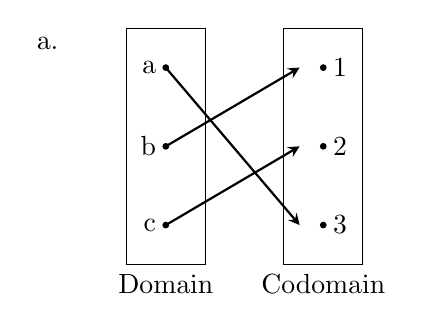
\begin{tikzpicture}[arrow/.style = {thick,-stealth}]
                    % Graph 1
                    \node [below] at (-1,3) {a.};
                    
                    \draw (0,0) rectangle (1,3);
                    \draw (2,0) rectangle (3,3);
                    
                    \node [below] at (0.5,0) {Domain};
                    \node [below] at (2.5,0) {Codomain};

                    \filldraw (0.5, 0.5) circle (1pt) node[left] {c};
                    \filldraw (0.5, 1.5) circle (1pt) node[left] {b};
                    \filldraw (0.5, 2.5) circle (1pt) node[left] {a};

                    \filldraw (2.5, 0.5) circle (1pt) node[right] {3};
                    \filldraw (2.5, 1.5) circle (1pt) node[right] {2};
                    \filldraw (2.5, 2.5) circle (1pt) node[right] {1};
                    
                    \draw[arrow] (0.5, 0.5) -- (2.2, 1.5);
                    \draw[arrow] (0.5, 1.5) -- (2.2, 2.5);
                    \draw[arrow] (0.5, 2.5) -- (2.2, 0.5);
                \end{tikzpicture}
                \solution{ Onto, one-to-one, and invertible. }{}
                &
                
                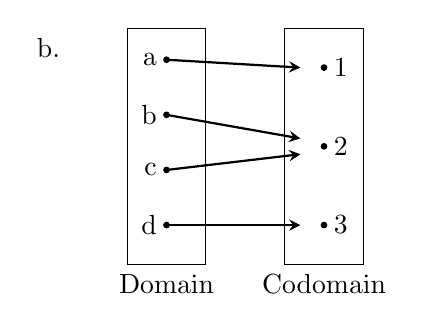
\begin{tikzpicture}[arrow/.style = {thick,-stealth}]
                    \node [below] at (-1,3) {b.};
                    
                    \draw (0,0) rectangle (1,3);
                    \draw (2,0) rectangle (3,3);
                    
                    \node [below] at (0.5,0) {Domain};
                    \node [below] at (2.5,0) {Codomain};

                    \filldraw (0.5, 2.6) circle (1pt) node[left] {a};
                    \filldraw (0.5, 1.9) circle (1pt) node[left] {b};
                    \filldraw (0.5, 1.2) circle (1pt) node[left] {c};
                    \filldraw (0.5, 0.5) circle (1pt) node[left] {d};

                    \filldraw (2.5, 0.5) circle (1pt) node[right] {3};
                    \filldraw (2.5, 1.5) circle (1pt) node[right] {2};
                    \filldraw (2.5, 2.5) circle (1pt) node[right] {1};
                    
                    \draw[arrow] (0.5, 0.5) -- (2.2, 0.5);
                    \draw[arrow] (0.5, 1.9) -- (2.2, 1.6);
                    \draw[arrow] (0.5, 1.2) -- (2.2, 1.4);
                    \draw[arrow] (0.5, 2.6) -- (2.2, 2.5);
                \end{tikzpicture}
                \solution{ Onto, not one-to-one, not invertible }{}

                \\
                
                \Square\ Onto \tab \Square\ One-to-one
                & \Square\ Onto \tab \Square\ One-to-one
                \\
                \Square\ Invertible & \Square\ Invertible

                \\ \hline \\

                
                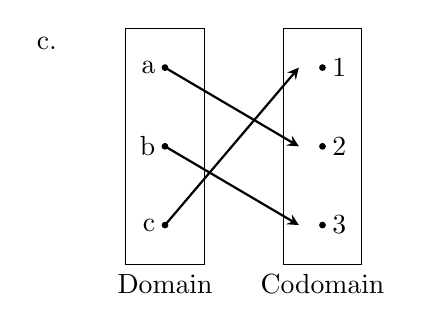
\begin{tikzpicture}[arrow/.style = {thick,-stealth}]
                    \node [below] at (-1,3) {c.};
                    
                    \draw (0,0) rectangle (1,3);
                    \draw (2,0) rectangle (3,3);
                    
                    \node [below] at (0.5,0) {Domain};
                    \node [below] at (2.5,0) {Codomain};

                    \filldraw (0.5, 0.5) circle (1pt) node[left] {c};
                    \filldraw (0.5, 1.5) circle (1pt) node[left] {b};
                    \filldraw (0.5, 2.5) circle (1pt) node[left] {a};

                    \filldraw (2.5, 0.5) circle (1pt) node[right] {3};
                    \filldraw (2.5, 1.5) circle (1pt) node[right] {2};
                    \filldraw (2.5, 2.5) circle (1pt) node[right] {1};
                    
                    \draw[arrow] (0.5, 0.5) -- (2.2, 2.5);
                    \draw[arrow] (0.5, 2.5) -- (2.2, 1.5);
                    \draw[arrow] (0.5, 1.5) -- (2.2, 0.5);
                \end{tikzpicture}
                \solution{ Onto, One-to-one, Invertible }{}
                &
                
                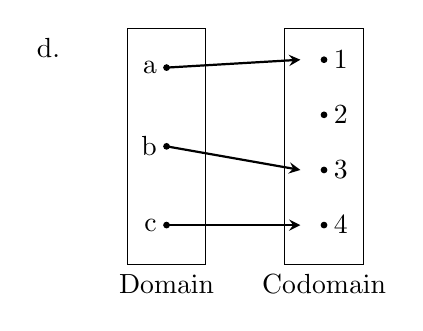
\begin{tikzpicture}[arrow/.style = {thick,-stealth}]
                    \node [below] at (-1,3) {d.};
                    
                    \draw (0,0) rectangle (1,3);
                    \draw (2,0) rectangle (3,3);
                    
                    \node [below] at (0.5,0) {Domain};
                    \node [below] at (2.5,0) {Codomain};

                    \filldraw (0.5, 0.5) circle (1pt) node[left] {c};
                    \filldraw (0.5, 1.5) circle (1pt) node[left] {b};
                    \filldraw (0.5, 2.5) circle (1pt) node[left] {a};

                    \filldraw (2.5, 2.6) circle (1pt) node[right] {1};
                    \filldraw (2.5, 1.9) circle (1pt) node[right] {2};
                    \filldraw (2.5, 1.2) circle (1pt) node[right] {3};
                    \filldraw (2.5, 0.5) circle (1pt) node[right] {4};
                    
                    \draw[arrow] (0.5, 2.5) -- (2.2, 2.6);
                    \draw[arrow] (0.5, 1.5) -- (2.2, 1.2);
                    \draw[arrow] (0.5, 0.5) -- (2.2, 0.5);
                \end{tikzpicture}
                \solution{ One-to-one, not onto, not invertible }{}

                \\
                \Square\ Onto \tab \Square\ One-to-one
                & \Square\ Onto \tab \Square\ One-to-one
                \\
                \Square\ Invertible & \Square\ Invertible

                \\ \hline \\
                
                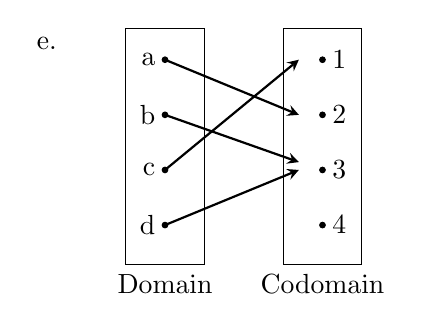
\begin{tikzpicture}[arrow/.style = {thick,-stealth}]
                    \node [below] at (-1,3) {e.};
                    
                    \draw (0,0) rectangle (1,3);
                    \draw (2,0) rectangle (3,3);
                    
                    \node [below] at (0.5,0) {Domain};
                    \node [below] at (2.5,0) {Codomain};

                    \filldraw (0.5, 2.6) circle (1pt) node[left] {a};
                    \filldraw (0.5, 1.9) circle (1pt) node[left] {b};
                    \filldraw (0.5, 1.2) circle (1pt) node[left] {c};
                    \filldraw (0.5, 0.5) circle (1pt) node[left] {d};

                    \filldraw (2.5, 2.6) circle (1pt) node[right] {1};
                    \filldraw (2.5, 1.9) circle (1pt) node[right] {2};
                    \filldraw (2.5, 1.2) circle (1pt) node[right] {3};
                    \filldraw (2.5, 0.5) circle (1pt) node[right] {4};
                    
                    \draw[arrow] (0.5, 0.5) -- (2.2,1.2);
                    \draw[arrow] (0.5, 1.2) -- (2.2,2.6);
                    \draw[arrow] (0.5, 2.6) -- (2.2,1.9);
                    \draw[arrow] (0.5, 1.9) -- (2.2,1.3);
                \end{tikzpicture}
                \solution{ Not onto, not one-to-one, not invertible }{}
                &
                
                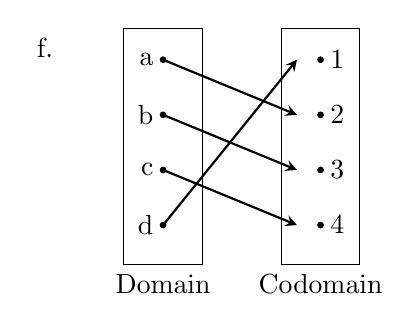
\begin{tikzpicture}[arrow/.style = {thick,-stealth}]
                    \node [below] at (-1,3) {f.};
                    
                    \draw (0,0) rectangle (1,3);
                    \draw (2,0) rectangle (3,3);
                    
                    \node [below] at (0.5,0) {Domain};
                    \node [below] at (2.5,0) {Codomain};

                    \filldraw (0.5, 2.6) circle (1pt) node[left] {a};
                    \filldraw (0.5, 1.9) circle (1pt) node[left] {b};
                    \filldraw (0.5, 1.2) circle (1pt) node[left] {c};
                    \filldraw (0.5, 0.5) circle (1pt) node[left] {d};

                    \filldraw (2.5, 2.6) circle (1pt) node[right] {1};
                    \filldraw (2.5, 1.9) circle (1pt) node[right] {2};
                    \filldraw (2.5, 1.2) circle (1pt) node[right] {3};
                    \filldraw (2.5, 0.5) circle (1pt) node[right] {4};
                    
                    \draw[arrow] (0.5,0.5) -- (2.2,2.6);
                    \draw[arrow] (0.5,1.2) -- (2.2,0.5);
                    \draw[arrow] (0.5,1.9) -- (2.2,1.2);
                    \draw[arrow] (0.5,2.6) -- (2.2,1.9);
                \end{tikzpicture}
                \solution{ Onto, one-to-one, invertible }{}

                \\
                
                \Square\ Onto \tab \Square\ One-to-one
                & \Square\ Onto \tab \Square\ One-to-one
                \\
                \Square\ Invertible & \Square\ Invertible
            \end{tabular}
        \end{center}

    \end{questionNOGRADE}

    \notonkey{ \newpage }{ \hrulefill }

    % -------------------------------------------------------------%
    % - QUESTION --------------------------------------------------%
    % -------------------------------------------------------------%
    \stepcounter{question}
    \begin{questionNOGRADE}{\thequestion}
            

        The function
        $ f : \mathbb{R} \to \mathbb{R}$, with the rule $f(x) = x^{2} + 4x + 1$ \\
        is not onto and not one-to-one.
        \begin{center}
            \begin{tikzpicture}
            \begin{axis}[
                axis lines = center,
                xlabel = $x$,
                ylabel = {$f(x)$},
                xmin=-10,
                xmax=3,
                ymin=-5,
                ymax=10,
                legend pos=south west,
            ]
            %Below the red parabola is defined
            \addplot [
                domain=-10:10, 
                samples=100, 
                color=red,
            ]
            {x^2 + 4*x + 1};
            \addlegendentry{$x^2 + 4x + 1$}
            \end{axis}
            \end{tikzpicture}
        \end{center}
        \begin{itemize}
            \item[a.]   Give an example of an element in the codomain
                        that has no element in the domain associated with it.
                        \solution{
                            There is no $x \in \mathbb{R}$ for which $f(x) = -4$
                            since the equation $x^{2} + 4x + 1 = -4$ has
                            no \textbf{real} solutions (by using the quadratic formula).
                        }{ \vspace{4cm} }

            \item[b.]   Given an example of two elements in the domain
                        that are both associated with the same output
                        in the codomain.
                        \solution{
                            $f(-1) = 1 - 4 + 1 = -2$ and $f(-3) = 9 - 12 + 1 = -2$.
                        }{ \vspace{3cm} }
        \end{itemize}
    \end{questionNOGRADE}






        
\end{document}








